%-----------------------------------------------------------------------------%
\chapter{\babDua}
%-----------------------------------------------------------------------------%
Bab ini menjelaskan tentang teori dan konsep yang digunakan dalam penelitian ini, di antaranya teori tentang \textit{weighted Voronoi diagram}, jarak Euclidean, \textit{hotspot}, dan lain-lain.

%-----------------------------------------------------------------------------%
\section{Diagram Voronoi}\label{sec:diagramVoronoi}
%-----------------------------------------------------------------------------%

Diagram Voronoi dari sekumpulan titik adalah diagram yang membagi suatu daerah menjadi bagian-bagian yang paling dekat dengan masing-masing titik tersebut \cite{geometric.algebra}.

\begin{figure}
	\centering
	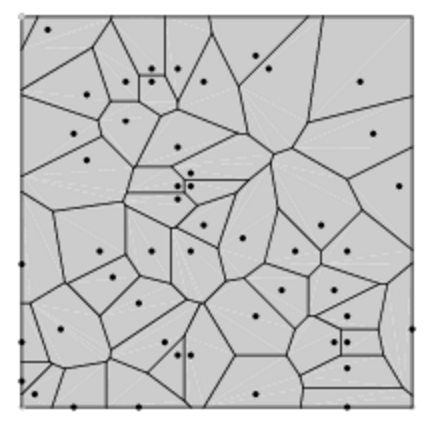
\includegraphics[width=6cm]{pics/diagramVoronoi.png}
	\caption{Diagram Voronoi}
	\label{fig:diagramVoronoi}
	\cite{diagram.voronoi}
\end{figure} 

\subsection{Contoh Aplikasi Diagram Voronoi}
\begin{enumerate}
\item Menggambarkan daerah yang didiami suatu pohon jika terdapat kumpulan pohon-pohon yang dilihat dari atas. \cite{voronoi.wiki}

\item Terdapat kumpulan pos ambulan di suatu kota, jika terdapat keadaan darurat di suatu tempat, dari pos manakah ambulan akan datang? \cite{voronoi.wiki}

\item Mengambil sampel jenis tanah di suatu daerah dan mengelompokkan jenis tanah masing-masing bagian berdasarkan sampel yang diambil. \cite{voronoi.wiki}
\end{enumerate}

\subsection{Macam-Macam Diagram Voronoi}
Menurut Okabe, dkk. \cite{spatial.tessellations} diagram Voronoi digeneralisasikan menjadi beberapa jenis sebagai berikut: 

\subsubsection{Weighted Voronoi Diagram}

Pada diagram Voronoi biasa secara implisit mengasumsikan bahwa setiap titik adalah identik (kecuali lokasinya) atau setiap titik memiliki bobot yang sama. Namun \textit{generator points} memiliki bobot yang berbeda yang mencerminkan sifat dari \textit{generator points} itu sendiri; sebagai contoh, ukuran populasi dari suatu pemukiman, jumlah fungsi-fungsi pada pusat perbelanjaan, jumlah emisi dari suatu polutan, ukuran dari sebuah atom pada suatu struktur kristal, dan lain-lain. 

Terdapat sekumpulan titik yang berbeda-beda, $\mathbb{P} = \left \{ p_{1},...,p_{n}\right \} \subset \mathbb{R}^{m} \left ( 2\leq n< \infty  \right ) \left ( A = P, S = \mathbb{R}^{m} \right )$ dan untuk masing-masing $p_{i}$ diberikan bobot yang sesuai dengan sifatnya. Kita representasikan bobot ini dengan sekumpulan parameter $\mathbb{W_{i}} = \left \{w_{i1},...,w_{in_{w}} \right \}$ (jika $n_{w} = 1$, kita tulis $w_{i}$ untuk $\mathbb{W_{i}}$). Dengan bobot ini kita definisikan jarak, $d_{w} \left(p,p_{i}\right)$, dari $p$ to $p_{i}$, disebut dengan sebuah \textit{weighted distance}. Daerah kekuasaan dari $p_{i}$ melalui $p_{j}$ dengan \textit{weighted distance}-nya ditulis dalam persamaan berikut:

\begin{equation} \label{eq1}
	Dom \left(p_{i},p_{j}\right)=\left \{p | d_{w}\left(p,p_{i}\right) \leq d_{w} \left(p,p_{j}\right) \right \}, j \neq i.
\end{equation}

dimana

\begin{equation} \label{eq2}
	V\left(p_{i}\right)=\bigcap_{i\in I_{n} \ \left {i \right }}^{} Dom \left(p_{i},p_{j}\right),
\end{equation}

dan $\mathbb{V} \left (P, d_{w}, \mathbb{R}^{m} \right ) = \mathbb{V}_{w} = \left \{ V \left(p_{1}\right),..., V\left(p_{n}\right ) \right \}$. $\mathbb{V}_{w}$ menghasilkan suatu \textit{generated Voronoi diagram}. Atau kita sebut $\mathbb{V}_{w}$ sebagai \textit{weighted Voronoi diagram} yang dihasilkan oleh $P$ dengan bobot $\left \{W_{1},...,W_{n} \right \}$, dan himpunan $V\left(p_{i}\right)$ merupakan \textit{weighted Voronoi region} yang berasosiasi dengan $p_{i}$. \cite{spatial.tessellations}

\textit{Weighted Voronoi diagram} merupakan pengembangan dari diagram Voronoi biasa. Berdasarkan definisi dari diagram Voronoi biasa, \textit{weighted Voronoi diagram} bisa didefinisikan sebagai berikut:

Terdapat $P = \left \{p_{1}, p_{2},...,p_{n}\right \}, 3 \leq n < \infty$ sebagai himpunan titik kontrol pada ruang Euclidean dua dimensi, $\lambda \left(i = 1,2,...,n\right)$ adalah bilangan asli, maka

\begin{equation} \label{eq3}
	V\left(p_{i},\lambda_{i}\right)=\left \{x \in V\left(p_{i},\lambda_{i}\right) | \frac{d\left (x,p_{i} \right )}{\lambda_{i}} \leq \frac{d\left (x,p_{j} \right )}{\lambda_{j}}, j = 1,2,...,n, j \neq i \right \}
\end{equation}

$d\left(p_{i},p_{j}\right)$ merepresentasikan jarak Euclidean di antara titik $p_{i}$ dan $p_{j}$, $p_{i} \neq p_{j}$, $i \neq j$, $i, j, \in \left \{1,2,...,n\right \}, x$ adalah sembarang titik di bidang tersebut.

Bidang dibagi menjadi $n$ bagian, \textit{weighted Voronoi diagram} adalah bidang yang dibagi oleh $V_{n}\left(p_{i},\lambda_{i}\right) \left(i = 1,2,...,n\right), \lambda_{i}$ adalah bobot dari $p_{i}$, seperti yang terlihat dalam gambar berikut, jumlah bobot dari titik.

\begin{figure}
	\centering
	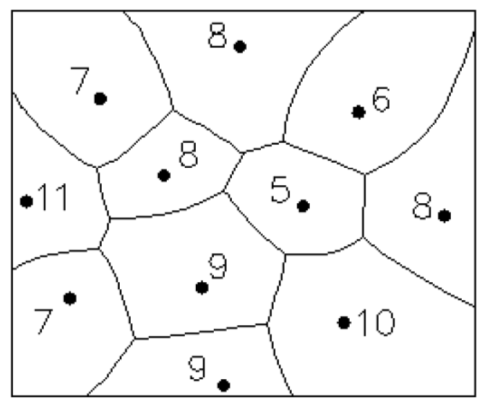
\includegraphics[width=6cm]{pics/weightedVoronoiDiagram.png}
	\caption{Weighted Voronoi Diagram}
	\label{fig:weightedVoronoiDiagram}
	\cite{substation}
\end{figure}

\textit{Weighted Voronoi graph} juga sesuai untuk segmentasi dari ruang. \textit{Weighted Voronoi diagram} digunakan untuk membagi ruang ketika terdapat perbedaan yang signifikan dari bobot untuk setiap titik. Ciri ini mengindikasikan bahwa bobot tersebut dapat digunakan untuk merefleksikan distribusi beban yang tidak sama dan efek-efek dari kapasitas dengan kadar yang berbeda dan kadar beban pada daerah yang dilayani oleh \textit{substation}.

Properti-properti dalam \textit{weighted Voronoi diagram}:

Dalam \textit{weighted Voronoi diagram}, $p_{i}, p_{j}$ merupakan dua \textit{occurrence elements} dengan sisi umum $l_{ij}$.

\begin{enumerate}
	\item Jika $\lambda_{i} = \lambda_{j}$, maka $l_{ij}$ adalah bagian dari garis vertikal dari segmen garis $p_{i}p_{j}$.
	\item Jika $\lambda_{i} \neq \lambda_{j}$, maka $l_{ij}$ adalah sebuah lingkaran atau lengkungan. Jika pusat dari garis lingkaran $l_{ij}$ adalah $O$, jari-jari $R$, koordinat $p_{i}$ adalah $\left(x_{i},y_{i}\right)$, koordinat dari $p_{j}$ adalah $\left(x_{j},y_{j}\right)$, $O, PI, PJ$ berada pada garis yang sama, dan
	\begin{enumerate}
		\item pusat koordinal adalah $\left(\frac{\lambda_{i}^{2} x_{j} - \lambda_{j}^{2} x_{i}}{\lambda_{i}^{2} - \lambda_{j}^{2}}, \frac{\lambda_{i}^{2} y_{j} - \lambda_{j}^{2} y_{i}}{\lambda_{i}^{2} - \lambda_{j}^{2}} \right)$;
		\item $R = \frac{\lambda_{i} \lambda_{j}}{| \lambda_{i}^{2} - \lambda_{j}^{2} |} d\left(p_{i},p_{j} \right)$;
		\item $d\left(O,p_{i} \right) = \frac{\lambda_{i}^{2}}{| \lambda_{i}^{2} - \lambda_{j}^{2} |} d\left(p_{i}, p_{j}\right)$, $d\left(O,p_{j} \right) = \frac{\lambda_{j}^{2}}{| \lambda_{j}^{2} - \lambda_{j}^{2} |} d\left(p_{i}, p_{j}\right)$
		\item $p_{i}, p_{j}$ adalah titik cermin dari lingkaran $O$
	\end{enumerate}
\end{enumerate} \cite{substation}

\subsubsection{Higher Order Voronoi Diagram}

Sebelum mengenal tentang \textit{higher order voronoi diagram}, kita perlu mengenal tentang \textit{first order voronoi diagram}. Terdapat sekumpulan titik $S$ pada bidang. Voronoi diagram dari $S$ adalah suatu dekomposisi dari suatu ruang ke dalam \textit{convex polygonal cells} (sel polihedral dalam dimensi yang lebih tinggi). Setiap titik $x$ dalam $S$ terkait dengan sebuah sel yang mengandung semua titik-titik dalam bidang tersebut yang lebih dekat dengan $x$ dari pada titik-titik lain dalam $S$. Sekumpulan sel kompleks ini adalah \textit{nearest neighbour decomposition.} \cite{hovd} 

\textit{Higher order voronoi diagram} mengekstend konsep diagram voronoi dengan mendefinisikan sel menggunakan $n$ \textit{nearest neighbour}. Sebagai contoh, jika $x$ dan $y$ adalah elemen yang berbeda dari $S$, maka terdapat suatu sekumpulan titik (yang kemungkinan besar kosong) yang mendefinisikan sebuah sel dalam diagram voronoi order kedua. tetangga terdekat dan tetangga terdekat kedua dari titik apapun dalam sel ini adalah $x$ dan $y$. Jumlah titik dalam $S$ yang mendefinisikan sebuah sel adalah order dari \textit{higher order voronoi diagram}.

Sebuah \textit{higher order voronoi diagram} (yang termasuk di dalamnya adalah \textit{first order voronoi diagram}) adalah sekumpulan sel yang membagi ruang. Bagaimanapun tidak seperti \textit{first order voronoi diagram}, \textit{dual} terhadap \textit{higher order voronoi diagram} tidak perlu membagi ruang. Sering terdapat kasus dimana segitiga dari \textit{higher order delaunay triangulation} akan memiliki persimpangan yang tidak kosong.

\subsubsection{Voronoi Diagrams with V-distances}

Voronoi diagram dapat digeneralisasi dengan jarak apapun selama jarak tersebut adalah V-distance. Jarak ini tidak harus jarak Euclidean. Seperti  \textit{multiplicatively weighted distance}, \textit{additively weighted distance}, \textit{compoundly weighted distance}, \textit{power distance} dan \textit{shortest-path distance}, yang mana bukan \textit{euclidean distance}, bisa membuat \textit{generalized voronoi diagram}. 

Voronoi diagram yang didefinisikan dengan Minkowski metriks dalam $R^m$. Minkowski (\textit{power}) metric dari suatu titik \textit{p} ke suatu titik $p_i$ dalam $R^m$ didefinisikan oleh

\begin{equation} \label{eqMinkowski}
d_L_p (p,p_i) = [\lambda_{j=1}^{m} | x_j - x_{ij} | ^ p]^{1/p}
\end{equation}

dimana ($x_1$,...,$x_m$) dan ($x_i1$,...,$x_im$) adalah koordinat Kartesian dari $p$ dan $p_i$, secara respektif. Secara random simbol $L_p$ adalah digunakan oleh metriks Minkowski, di mana $p$ merujuk pada derajat dari pangkat. Parameter $p$ berada pada range $1 \leq p < \infty$ . Jika $p = 1$, rumus \label{eqMinkowski} menjadi

\begin{equation} \label{manhattan}
d_L_1 (p, p_i) = \lambda_{j=1}^{m} | x_j - x_{ij} |
\end{equation} 

yang mana disebut dengan Manhattan metriks, \textit{city-block distance} atau \textit{taxi-cab distance}. Jika p=2, Minkowski metric adalah \textit{euclidean distance}. Jika $p = \infty$, Minkowski metric disebut dengan supremum metric atau dominance metric. \cite{spatial.tessellations}

\begin{figure}
	\centering
	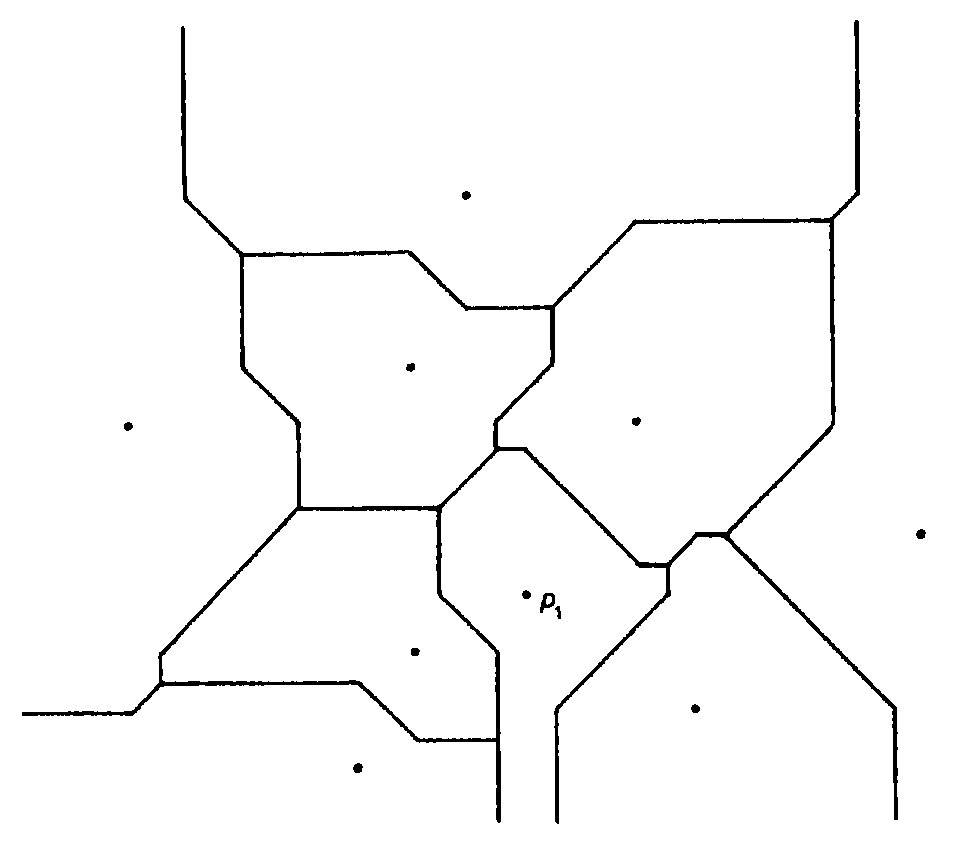
\includegraphics[width=10cm]{pics/manhattanVoronoiDiagram.png}
	\caption{Manhattan Voronoi Diagram}
	\label{fig:manhattanVoronoiDiagram}
	\cite{spatial.tessellations}
\end{figure}

\subsubsection{Network Voronoi Diagram}

Manhattan Voronoi diagram atau Karlsruhe Voronoi diagram berguna untuk menginvestigasi daerah yang dominan dalam sebuah \textit{grid street system} atau \textit{radial-circular street system}. Pada jalanan yang sesungguhnya, bahkan di Manhattan pun jalanan tidak sepenuhnya membentuk suatu grid. 

Terdapat \textit{planar geometric graph} G(N, L) terdiri dari sekumpulan nodes $N = {p_1,...,p_n,p_n+1,...,pl}$ dan sekumpulan links $L = {l_1,...,l_k}$ yang membentuk sebuah \textit{connected component}. Untuk menyederhanakan G(N,L) diasumsikan sebagai \textit{non-directed graph} (mengekstensi menjadi \textit{directed graph} tidak sulit). Pada G(N,L) mendefinisikan jarak dari sebuah titik p pada suatu link dalam L ke suatu node $p_i$ dalan N dengan jarak terpendeknya adalah dari p ke $p_i$.

\subsubsection{Voronoi Diagram for Moving Points}
Untuk jenis Voronoi diagram sebelumnya kita mengasumsikan bahwa lokasi dari generator adalah tetap sepanjang waktu. Dalam seksi ini diperhitungkan sebuah voronoi diagram yang dibuat dari sekumpulan titik yang selalu bergerak sepanjang waktu, atau secara umum merupakan sekumpulan titik yang lokasinya ditentukan oleh satu parameter.

\section{Macam-Macam Distances}

\subsection{Jarak Euclidean}
Jarak euclidean atau metriks euclidean adalah garis lurus biasa yang menghubungkan antara dua titik dalam \textit{euclidean space}. Dengan jarak ini \textit{euclidean space} menjadi \textit{metrics space}. \textit{Norm} (panjang) yang berhubungan dinamakan \textit{euclidean norm}. \textit{Euclidean distance} antara titik $p$ dan $q$ adalah panjang dari segmen garis yang menghubungkan mereka ($pq$).

Dalam koordinat kartesian, jika $p = (p_1, p_2, ..., p_n)$ dan $q = (q_1, q_2, ..., q_n)$ adalah dua titik dalam \textit{n}-ruang Euclidean, kemudian jarak (d) dari $p$ ke $q$, atau dari $q$ ke $p$ ditunjukkan oleh teorema Pythagoras:

\begin{equation} \label{euclidean}
	d(p, q) = d(q, p) = \sqrt{{\left (q_1 - p_1 \right )^2} + {\left (q_2 - p_2 \right )^2} + ... + {\left (q_n - p_n \right )^2}}
	= \sqrt{\sum_{i = 1}^{n} {(q_i - p_i)}^2}
\end{equation} 

Posisi dari sebuah titik dalam \textit{n}-ruang Euclidean adalah sebuah vektor Euclidean. Sehingga, $p$ dan $q$ adalah vektor-vektor Euclidean, yang dimulai dari sumber dari ruang, dan ujungnya mengarah pada dua titik. Euclidean \textit{norm} atau panjang Euclidean atau besar dari vektor menghitung panjang dari vektor:

\begin{equation}
	\left \| p \right \| = \sqrt{{p_1}^2 + {p_2}^2 + ... + {p_n}^2} = \sqrt{p.p}
\end{equation}

yang mana persamaan terakhir merupakan \textit{dot product}. \cite{euclidean.wiki}

\subsection{Chebyshev Distance}
\textit{Chebyshev distance} atau \textit{Tchebychev distance} adalah didefinisikan dalam metriks vektor dimana jarak antara 2 vektor adalah paling besar dari perbedaan mereka sepanjang dimensi koordinat apapun. 

	Disebut juga \textit{chessboard distance}. Dalam permainan catur jumlah pergerakan minimum dari king untuk berpindah dari satu kotak ke kotak lain setara dengan jarak Chebyshev antara titik pusat persegi ke titik pusat persegi lain jika sisi perseginya berukuran satu seperti yang direpresentasikan dalam koordinat spatial 2D dengan sumbu yang berada di tepi papan. Contohnya \textit{Chebyshev distance} antara f6 dan e2 adalah 4.
	
	Jarak Chebyshev antara dua vektor atau titik $p$ dan $q$, dengan standar koordinat $p_i$ dan $q_i$, adalah
	
\begin{equation}
	D_{Chebyshev}\left ( p,q \right ) := \underset{i}{max}\left ( \left | p_{i} - q_{i} \right | \right )
\end{equation}	 

Persamaan tersebut setara dengan limit dari metriks $L_p$:

\begin{equation}
\underset{k\rightarrow \infty }{lim} {\left ( \sum_{i = 1}^{n} {\left | p_i - q_i \right |}^{k}\right )}^{\frac{1}{k}}
\end{equation}

atau biasa disebut dengan metriks $L_\infty$.

	Secara matematika, jarak Chebyshev adalah metriks yang diinduksi oleh \textit{supremum norm} atau \textit{uniform norm}. Yang merupakan contoh dari metriks injektif.
	
	Dalam ruang dua dimensi, misalnya bidang, jika titik $p$ dan $q$ memiliki koordian Kartesian ($x_1, y_1$) dan ($x_2, y_2$), jarak Chebyshev-nya adalah
	
	\begin{equation}
	D_{Chess} = max \left ( \left | x_2 - x_1 \right |, \left | y_2 - y_1 \right | \right )
	\end{equation}
	
	Di bawah metriks tersebut, sebuah lingkaran dengan jari-jari $r$, yang mana kumpulan titik dengan jarak Chebyshev $r$ dari titik pusat, adalah sebuah persegi yang mana sisinya memiliki panjang $2r$ dan sejajar dengan sumbu koordinat $x$. \cite{chebyshev.wiki}

\subsection{Manhattan distance}
\textit{Manhattan distance} antara dua titik $x$ dan $y$ di ruang $n$ dimensi adalah jumlah jarak untuk masing-masing dimensi. Disebut Manhattan karena ini menggambarkan jarak suatu mobil yang berkendara dalam suatu kota (contoh Manhattan) dimana gedung-gedung ditata dalam blok-blok persegi dan jalan yang lurus memotong pada sudut kanan. L1 dan 1-\textit{norm distance} adalah deskripsi matematik untuk \textit{distance} ini.

\subsection{Mahalanobis Distance} 

Mahalonobis distance adalah jarak antara sebuah titik P dan sebuah distribusi D yang dikenalkan oleh P. C. Mahalonobis pada tahun 1936. Ini adalah generalisasi multi dimensi dari ide menghitung berapa banyak standar deviasi P dari rata-rata D. Jaraknya akan nol jika P berada pada rata-rata D, dan akan meningkat selama P menjauhi rata-rata dari D. Sepanjang setiap komponen utama dari sumbu, ini menghitung jumlah dari standar deviasi dari P ke rata-rata dari D. Jika setiap sumbu di skala ulang sehingga memiliki variansi unit, jarak Mahalonobis sebanding dengan jarak Euclidean standar pada ruang transformasi. Mahalonobis distance tidak memiliki unit dan skala nya tidak bervariasi, dan memperhitungkan hubungan dari data set. \cite{mahalanobis}

%-----------------------------------------------------------------------------%
%\section{Metode Perhitungan}\label{sec:metodePerhitungan}
%-----------------------------------------------------------------------------%

%-----------------------------------------------------------------------------%
\section{Menentukan Jumlah \textit{Station} Baru}\label{sec:jumlahStationBaru}
%-----------------------------------------------------------------------------%

Dalam paper Xiaojun dkk, metode yang digunakan untuk menghitung kuantitas dan kapasitas dari \textit{substation} adalah menghitung jumlah \textit{stations} baru, menghitung kapasitas dari \textit{station} baru, dan menggunakan \textit{weighted Voronoi diagram}.

Berdasarkan jumlah beban dari target, kapasitas dari \textit{station} saat ini dan himpunan kapasitas dari calon \textit{substation}, jumlah maksimum dari $n\left(max\right)$ dan jumlah minimum dari $n\left(min\right)$ dan jumlah \textit{substation} baru (\textit{n}) bisa ditentukan dengan persamaan \ref{eq4} dan \ref{eq5}, yang mana di bawah kondisi \textit{power supply}.

\begin{equation} \label{eq4}
	n_{max} = \frac{\sum W - \sum P}{\left ( S_{e} \right)_{min} cos \varphi} + \eta
\end{equation}

\begin{equation} \label{eq5}
	n_{min} = \frac{\sum W - \sum P}{\left ( S_{e} \right)_{max} cos \phi}
\end{equation}

\begin{figure}
	\centering
	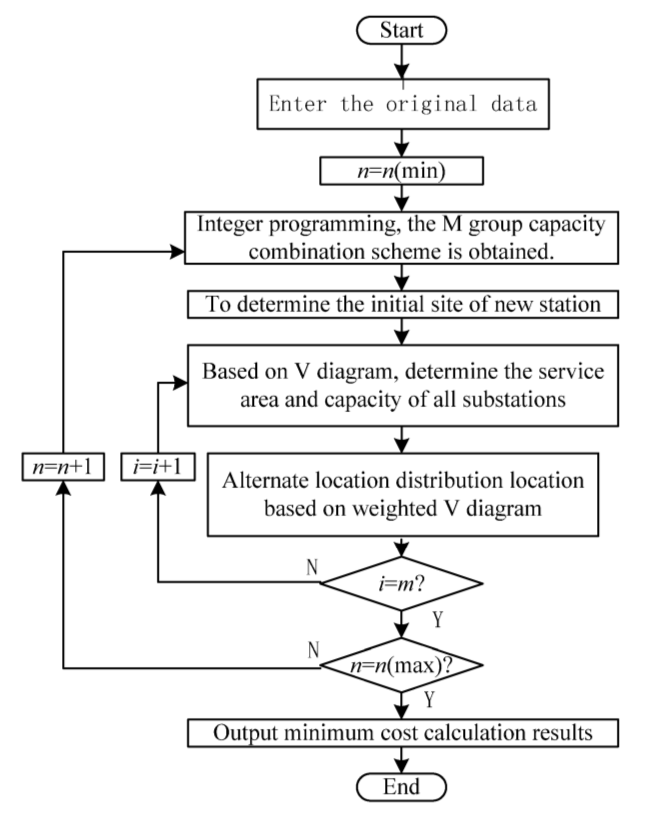
\includegraphics[width=10cm]{pics/substationPlanning.png}
	\caption{Flow Chart dari Substation Planning}
	\label{fig:substationPlanning}
	\cite{substation}
\end{figure}

$\sum W$ adalah jumlah muatan aktif dari seluruh muatan; $\sum P$ adalah jumlah kapasitas daya aktif dari \textit{transformer substation} dalam tahun (termasuk ekspansi dari kapasitas \textit{station} saat ini); $S\left(Se\right)_{max} = max\left \{S_{i}e \left(S_{i}\right) | S_{i} \in Q \right \}$ adalah nilai maksimum kapasitas ekonomi (kapasitas x \textit{load ratio}) dalam tipe kandidat untuk \textit{substation}; $\left(Se\right)_{min}$ adalah kapasitas ekonomi minimum dari tipe kandidat dari \textit{substation}; $\eta$ adalah \textit{relaxation factor}.

%-----------------------------------------------------------------------------%
%\subsection{Menentukan Kapasitas dari Substation Baru}\label{sec:kapasitasStationBaru}
%%-----------------------------------------------------------------------------%
%
%Jika jumlah dari \textit{station} baru adalah $n$, kita dapat menentukan m grup kombinasi dari kapasitas \textit{station} baru berdasarkan kapasitas dari \textit{transformer substation} yang baru dan kapasitas dari \textit{station} saat ini pada tahun yang telah ditargetkan. Dapat dibentuk model matematika seperti berikut:
%
%\begin{figure}
%	\centering
%	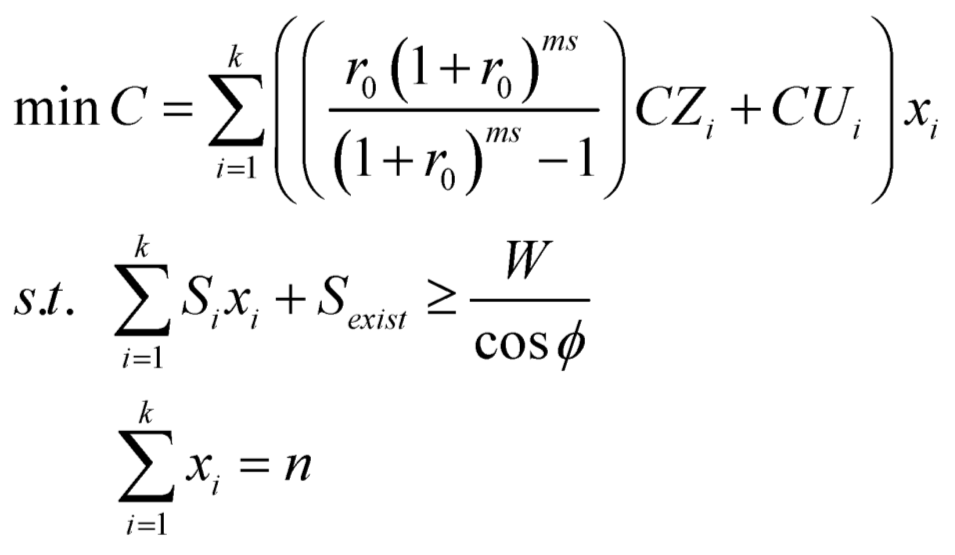
\includegraphics[width=9cm]{pics/formula.png}
%	\label{eq6}
%	\cite{substation}
%\end{figure}
%
%$k$ adalah jumlah dari tipe kandidat \textit{transformer substation}; $CZ_{i}$ adalah biaya investasi dari $i$ kandidat tipe \textit{transformer substation}; 

%-----------------------------------------------------------------------------%
\section{Hotspot}\label{sec:hotspot}
%-----------------------------------------------------------------------------%

%- Menghitung kapasitas suatu hotspot (kapasitas ini bisa kekuatan si hotspot atau luas area jangkauannya)

%- penempatan hotspot di suatu ruang terbuka
% Untuk open area tinggal ngitung 100m jari2 dari pusat (atau diameter?). kalo misal UI dianggap open area, berarti bikin lingkaran2 per 100 m, (minus danau dan hutan)

\textit{Wi-Fi hotspot} adalah \textit{wireless access point} yang menyediakan jaringan atau akses internet untuk perangkat \textit{mobile} seperti \textit{laptop} atau \textit{smartphone}, yang biasanya terdapat di tempat-tempat umum.  

Wi-Fi digunakan untuk menyediakan akses internet untuk perangkat yang berada dalam jangkauan dari jaringan nirkabel yang terhubung dengan internet. Cakupan dari satu atau lebih \textit{hotspot-hotspot} yang saling berhubungan bisa diperluas dari suatu area yang hanya seluas sebuah kamar hingga seluas beberapa kilometer persegi. Cakupan dalam daerah yang lebih luas membutuhkan sekumpulan \textit{access point} dengan cakupan yang saling tumpang tindih. Contohnya teknologi \textit{public outdoor Wi-Fi} yang telah berhasil diimplementasikan dalam \textit{wireless mesh network}.

\textit{Wireless Mesh Network} (WMN) adalah jaringan komunikasi yang terdiri dari \textit{radio nodes} yang terorganisir dalam \textit{mesh topology}. WMN terdiri dari \textit{mesh clients}, \textit{mesh routers} dan \textit{gateways}. 

\textit{Mesh clients} merupakan perangkat yang menggunakan jaringan nirkabel tersebut, seperti laptop, telefon seluler, dan perangkat-perangkat nirkabel lainnya. \textit{Mesh routers} digunakan untuk meneruskan arus baik dari atau menuju ke \textit{gateways}. \textit{Router} bisa terhubung atau tidak terhubung ke internet. 

\section{GIS}
\textit{still don't know why we need this}

\section{Tools}
Terdapat beberapa \textit{tools} yang dapat digunakan untuk mengimplementasikan \textit{weighted Voronoi diagram}, diantaranya: R studio, ArcGIS, WVD18, java library, dan lain-lain.

\subsection{R Studio}

%R studio 
%https://www.stat.auckland.ac.nz/~paul/Reports/VoronoiTreemap/voronoiTreeMap.html

RStudio adalah Integrated Development Environment (IDE) untuk R yang didalamnya terdapat console, syntax-highlighting editor yang mendukung eksekusi kode secara langsung, melakukan plotting, melihat history, debugging, dan manajemen \textit{workspace}.

Kelebihan dari tools ini adalah dapat melakukan perhitungan voronoi diagram serta melakukan \textit{plotting} dari diagram.

\subsection{ArcGIS}
ArcGIS adalah \textit{platform} yang digunakan untuk melakukan pemetaan dan analisis. ArcGIS dapat melakukan untuk melakukan analisis spasial, pemetaan dan visualisasi, menggambarkan GIS 3D, \textit{real time} GIS, perbandingan dan \textit{remote sensing}, serta pengumpulan dan managemen data. \cite{arcgis}

\subsection{OpenVoronoi}

OpenVoronoi adalah suatu tools yang menghitung voronoi diagram 2D untuk titik, garis lurus dan garis lengkung. Kekurangan dari tools ini adalah belum mengeluarkan output berupa gambar. Perlu ditambahkan beberapa program untuk menghasilkan gambar diagram voronoinya. \cite{open.voronoi}

\subsection{Java Library: Power Voronoi Diagram}

Power Voronoi Diagram merupakan Java Library yang menghitung suatu weighted voronoi diagram yang disebut Power Diagram. Perbedaan utama dengan voronoi diagram biasa adalah kemungkinan untuk memberikan bobot positif untuk setiap situs yang akan mempengaruhi sel-sel voronoi yang berkaitan. Jika bobot tersebut diberi nilai nol, maka hasilnya merupakan diagram voronoi biasa. \cite{power.voronoi.diagram}

Java Library ini hanya melakukan perhitungan dan pembuatan diagram voronoi tanpa melakukan penggambaran diagramnya.

%-----------------------------------------------------------------------------%
\section{Peta Kampus Universitas Indonesia}\label{sec:petaUI}
%-----------------------------------------------------------------------------%

Kampus Universitas Indonesia Depok memiliki luas 320 hektar yang terdiri dari 75 persen area hijau seperti hutan dan danau \cite{ui}. 25 persennya terdiri dari fakultas-fakultas dan jalan yang menghubungkan antarfakultas. 

Selain fakultas, dalam area kampus UI Depok juga terdapat fasilitas umum seperti perpustakaan, stasiun, asrama, rektorat, dan lain-lain.

\begin{figure}
	\centering
	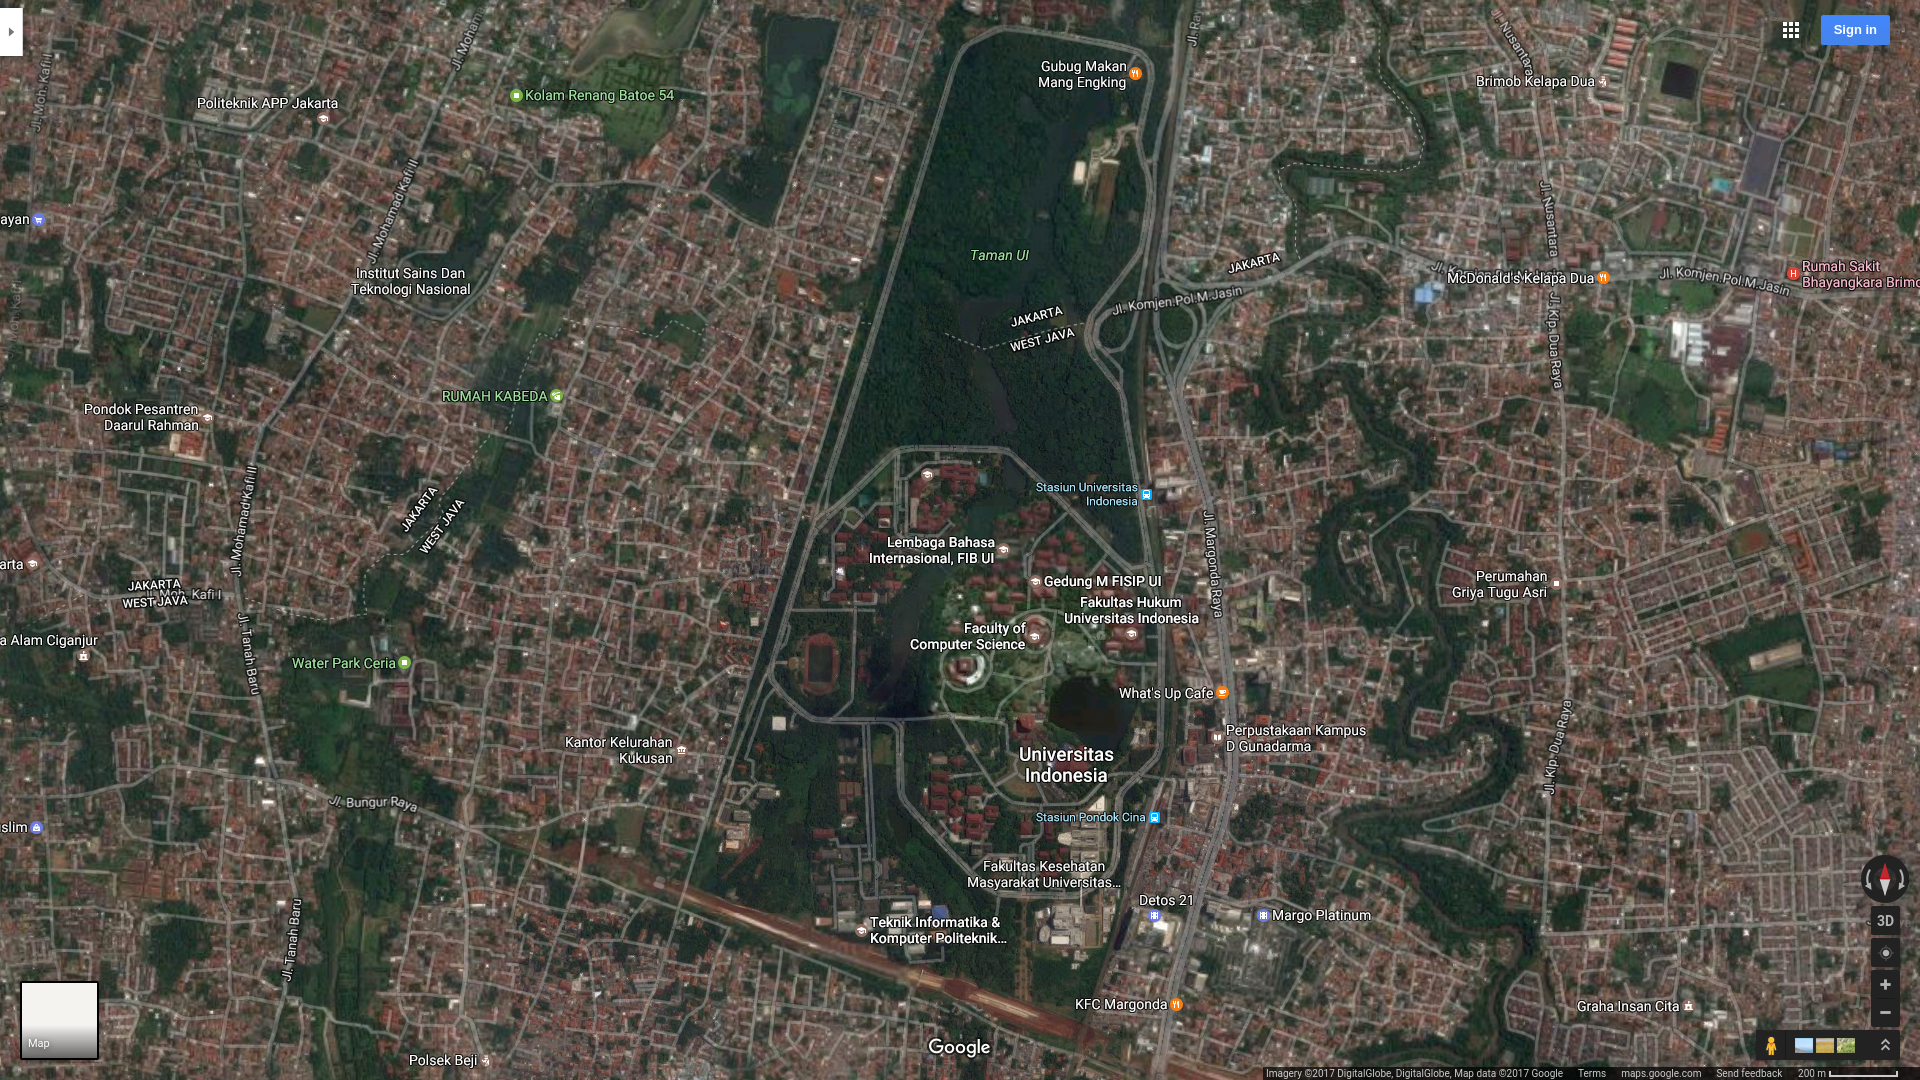
\includegraphics[width=14cm]{pics/ui-map.png}
	\caption{Peta Kampus Universitas Indonesia Depok}
	\label{fig:UImap}
	\cite{ui.map}
\end{figure}

Universitas Indonesia terdiri atas 47.641 mahasiswa (tahun 2015) yang tersebar dalam 14 fakultas yang tergolong dalam tiga rumpun, yaitu Rumpun Ilmu Kesehatan (RIK), Rumpun Sains-Teknologi (Saintek), dan Rumpun Sosial-Humaniora (Soshum). \cite{ui.wiki}

Yang termasuk dalam Rumpun Ilmu Kesehatan adalah:
\begin{itemize}
 \item Fakultas Kedokteran
 \item Fakultas Kedokteran Gigi
 \item Fakultas Farmasi
 \item Fakultas Kesehatan Masyarakat
 \item Fakultas Ilmu Keperawatan
\end{itemize}

Rumpun Sains-Teknologi:
\begin{itemize}
\item Fakultas Matematika dan Ilmu Pengetahuan Alam
\item Fakultas Teknik
\item Fakultas Ilmu Komputer
\end{itemize}

Rumpun Sosial-Humaniora:
\begin{itemize}
\item Fakultas Hukum
\item Fakultas Ekonomi dan Bisnis
\item Fakultas Ilmu Pengetahuan Budaya
\item Fakultas Psikologi
\item Fakultas Ilmu Sosial dan Ilmu Politik
\item Fakultas Ilmu Administrasi
\end{itemize}

\section{WiFi 101}

WiFi adalah sebuah teknologi untuk \textit{wireless local area networking} dengan \textit{device} yang menggunakan standar IEEE 802.11. WiFi adalah merek dagang dari Wi-Fi Alliance, yang membatasi penggunaan term WiFi Certified dengan produk yang telah menyelesaikan tes sertifikasi \textit{interoperabilility}. \cite{wifi}

\textit{Device} yang bisa menggunakan teknologi WiFi diantaranya \textit{personal computer}, \textit{video-game console}, \textit{handphone} dan \textit{tablet}, kamera digital, \textit{smart} TV, \textit{digital audio player}, dan printer modern. \textit{Device} yang kompatibel dengan WiFi bisa terhubung dengan internet melalui WLAN dan \textit{wireless access point}. Sebuah akses poin atau \textit{hotspot} memiliki jarak sekitar 20 meter untuk \textit{indoor} dan jaraknya lebih jauh untuk \textit{outdoor}. Jangkauan \textit{hotspot} bisa sekecil satu ruangan dengan dinding yang memblokir gelombang radio, dan bisa seluas beberapa kilometer persegi yang bisa dicapai dengan menggunakan beberapa \textit{overlapping access point}.

WiFi biasanya menggunakan frekuensi radio 2.4 \textit{gigahertz} (12 cm) UHF dan 5.8 \textit{gigahertz} (5 cm) SHF ISM. Siapapun yang berada dalam jangkauan tersebut dan menggunakan \textit{modem wireless} bisa mengakses jaringan tersebut. Karena hal itu, WiFi lebih rentan untuk diserang (yang disebut dengan \textit{eavesdropping}) dibandingkan dengan jaringan kabel.